
\hypertarget{working_tools}{}
\section{Tools interface}
\index{tools}
\index{tools!interface}

This graphical interface
(Figure \ref{fig:tools_misc_options})
was projected to allow access to Tinn-R resources
and also to accommodate future growth of related news resources.

Position: starting from version 2.1.1.1 (Oct/15/2008) this interface is
dockable. It can float or be docked on the left, top, right, or bottom
sides of the main interface.

%% Misc
%-------------------------------------------------------------------------
\hypertarget{working_tools_misc}{}
\subsection{Misc (Tools)}
\index{tools!misc}

\begin{figure}[H]
  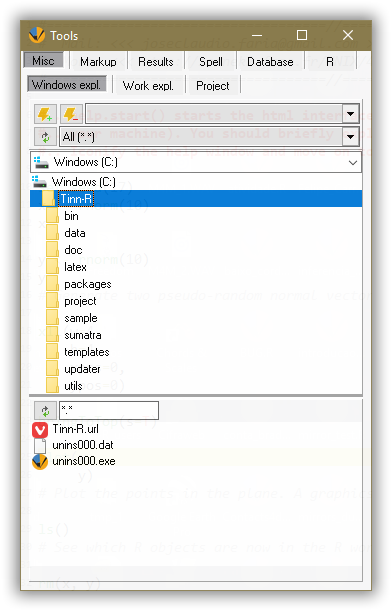
\includegraphics[scale=0.35]{./res/tools_misc_windowsexpl.png}~~
  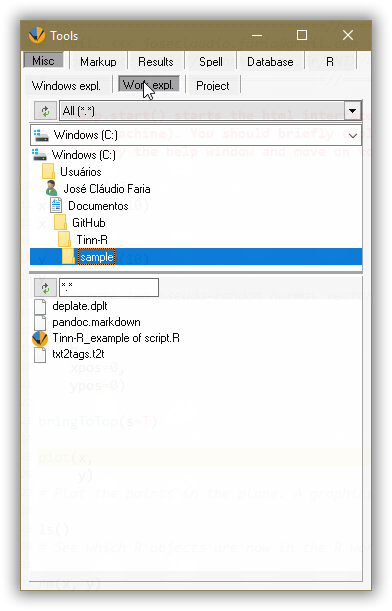
\includegraphics[scale=0.35]{./res/tools_misc_workexpl.png}~~
  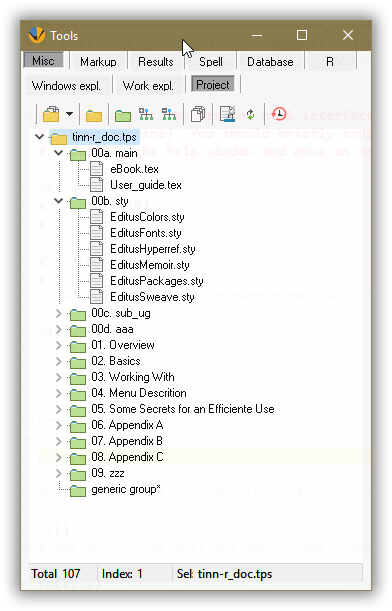
\includegraphics[scale=0.35]{./res/tools_misc_project.png}\\
  \caption{Tools interface.}
  \label{fig:tools_misc_options}
\end{figure}
%-------------------------------------------------------------------------

\begin{table}[H]
  \begin{footnotesize}
    \begin{tabularx}{\textwidth}{>{\hsize=0.3\hsize}X>{\hsize=0.7\hsize}X}\\
      \hline
      \textbf{Tool} & \textbf{Description} \\
      \hline
      Windows expl. & \textit{\href{\#working\_tools\_misc\_windowsexpl}{See details ...}} \\
      Work expl. & \textit{\href{\#working\_tools\_misc\_workexpl}{See details ...}} \\
      Project & \textit{\href{\#working\_tools\_misc\_project}{See details ...}} \\
      \hline
    \end{tabularx}
  \end{footnotesize}
  \caption{Misc (tools)}
  \label{tab:tools_misc}
\end{table}

The resources are showed in
Figure \ref{fig:tools_misc_options} and
Table \ref{tab:tools_misc}.


%% Windows expl.
%-------------------------------------------------------------------------
\hypertarget{working_tools_misc_windowsexpl}{}
\subsubsection{Windows expl.:}\\
\index{tools!Windows expl.}
%-------------------------------------------------------------------------

See Figure \ref{fig:tools_misc_options}.

\begin{itemize}
  \item Allows manager favorites (add and remove);
  \item Allows filter by file extension;
  \item Has pop-up menus similar to Windows explorer;
  \item Support drag and drop actions (it is possible to drag
    any file and drop it on the editor interface to be opened).
\end{itemize}


%% Work expl.
%-------------------------------------------------------------------------
\hypertarget{working_tools_misc_workexpl}{}
\subsubsection{Work expl.:}\\
\index{tools!Work expl.}
%-------------------------------------------------------------------------

See Figure \ref{fig:tools_misc_options}.

\begin{itemize}
  \item Always shows the folder related to the latest file opened;
  \item Does not have a pop-up menu;
  \item Supports drag and drop actions, i.e, it is possible to drag any
    file and drop it in the editor interface that will be opened.
\end{itemize}


%% Project
%-------------------------------------------------------------------------
\hypertarget{working_tools_misc_project}{}
\subsubsection{Project:}\\
\index{project}
\index{tools!project}
%% Project
%-------------------------------------------------------------------------

See Figure \ref{fig:tools_misc_options}.

\begin{itemize}
  \item Allows for project management using a graphical interface;
  \item Supports drag and drop actions, ie, it is possible to drag
    the entire project, groups, or any file and then drop them
    into the editor interface that will be opened:
    \begin{itemize}
      \item Project: will open all files related to the current project;
      \item Group: will open all files for the selected group;
      \item File: will open the selected file.
    \end{itemize}
  \item It is possible to send an entire project,
    a selected group, or an individual file to the \RR{} environment through a pop-up menu.
  \item  Source file of project:
    \begin{itemize}
      \item It is possible to edit the project in text mode (with the button
        \textit{Project: edit (as text file)} of the specific toolbar).
        After any change, save the text file (it contains the textual
        description of the project structure) and reload the file to the
        graphical interface (with the button \textit{Project:
          reload (from text file)} of the specific toolbar).
      \item Any changes to the graphical interface will be reflected in the
        text file for the project, after it is saved.
      \item The best way to work with projectis (graphics of textual mode)
        depends on the complexity of the actions and the user preference.
        For single tasks, we suggest that you use the graphical mode.
        For complex actions, it is faster to use the textual mode with
        all editor resources.
    \end{itemize}
\end{itemize}


%% Markup
%-------------------------------------------------------------------------
\hypertarget{working_tools_markup}{}
\subsection{Markup (Tools)}
\index{markup}
\index{tools!markup}
\index{tools!markup txt2tags}
\index{tools!markup \LaTeX}
%-------------------------------------------------------------------------

\begin{figure}[H]
  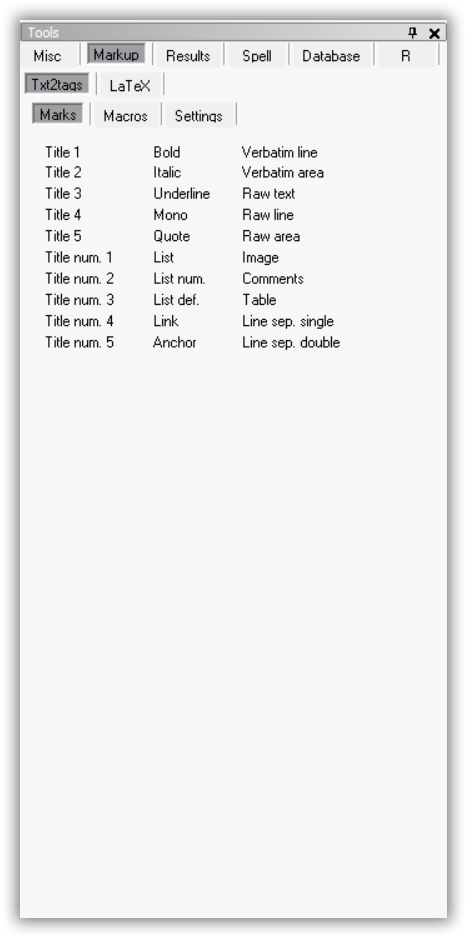
\includegraphics[scale=0.35]{./res/tools_markup_txt2tags_marks.png}~~
  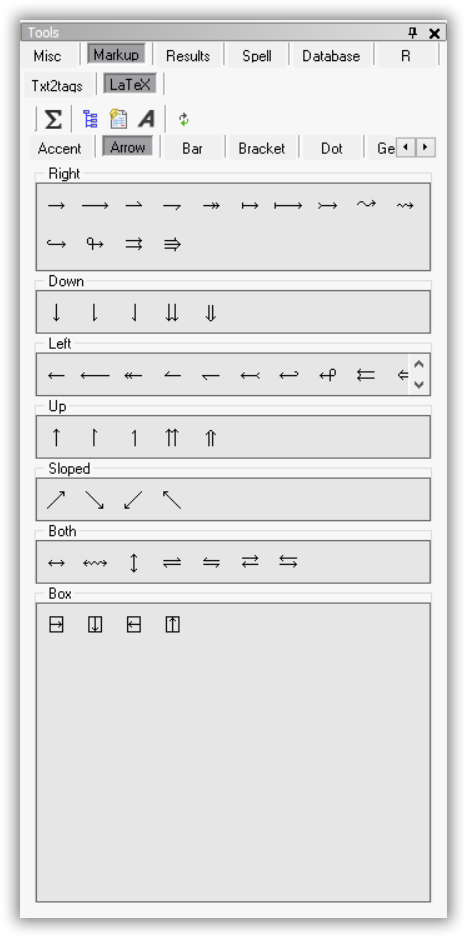
\includegraphics[scale=0.35]{./res/tools_markup_latex_arrows.png}\\
  \caption{Markups (Tools).}
  \label{fig:tools_markup_txt2tags_options}
\end{figure}

\begin{table}
  \begin{footnotesize}
    \begin{tabularx}{\textwidth}{lX}\\
      \hline
      \textbf{Tool} & \textbf{Description} \\
      \hline
      Txt2tags & Sets marks, macros and settings of Txt2tags convertor \\
      \LaTeX & Sets \LaTeX~symbols settings in a customizable manner \\
      \hline
      \\
    \end{tabularx}
  \end{footnotesize}
  \caption{Markup (Tools).}
  \label{tab:tools_markup}
\end{table}

It contains resources
(Figure \ref{fig:tools_markup_txt2tags_options} and
Table \ref{tab:tools_markup})
related to the Txt2tags and \LaTeX.


\subsubsection{Txt2tags:}\\
Sets
(Figure \ref{fig:tools_markup_txt2tags_options})
marks, macros, and settings for the Txt2tags convertor.
A single click over any graphical will add it to the current editor.


\subsubsection{\LaTeX:}\\
Set
(Figure \ref{fig:tools_markup_txt2tags_options})
of \LaTeX~symbols. A single click over any graphical object
will add it to the current editor;

The symbols, place and order of all symbols are customizable.
To customize them, open the folder \textit{latex} and edit
\textit{ini} path. At the end of the edition, update the interface
using the button \textit{Latex: reload symbols (from ini)}. Be careful
when editing the symbols to maintain the name structure.
For example: \texttt{Number\_SymbolName.FileExtension},
\texttt{001\_alpha.gif}, \texttt{002\_beta.gif}. The number
will be used to order symbols in the graphical interface,
while the name will be used (if recognized) as a \LaTeX~symbol.


%% Results
%-------------------------------------------------------------------------
\hypertarget{working_tools_results}{}
\subsection{Results (Tools)}
\index{tools!results}
%-------------------------------------------------------------------------

\begin{table}
  \begin{footnotesize}
    \begin{tabularx}{\textwidth}{>{\hsize=0.3\hsize}X>{\hsize=0.7\hsize}X}\\
      \hline
      \textbf{Tool} & \textbf{Description} \\
      \hline
      Ini log & Displays useful results when starting Tinn-R \\
      Search & Interface for \textit{Search} results associated with \textit{Search in files} \\
      Hex viewer & Interface for hex viewer \\
      \hline
      \\
    \end{tabularx}
  \end{footnotesize}
  \caption{Results (Tools).}
  \label{tab:tools_results}
\end{table}

It contains resources
(Table \ref{tab:tools_results})
related to \textit{Ini log}, \textit{Search} and \textit{Hex viewer}.


%% Ini log
%-------------------------------------------------------------------------
\subsubsection{Ini log:}\\
\index{tools!results inilog}

\begin{figure}[H]
  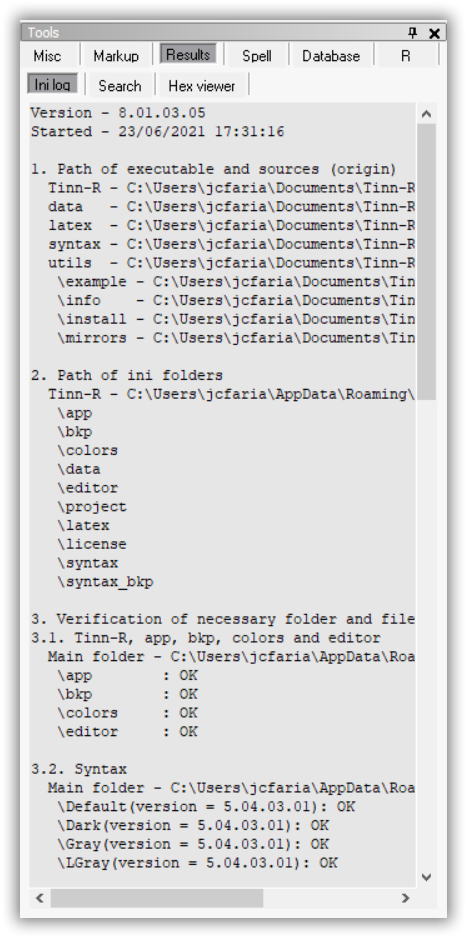
\includegraphics[scale=0.35]{./res/tools_results_inilog.png}\\
  \caption{Inilog (Tools/Results).}
  \label{fig:tools_results_inilog}
\end{figure}
%-------------------------------------------------------------------------

\begin{table}
  \begin{footnotesize}
    \begin{tabularx}{\textwidth}{XX}\\
      \hline
      \textbf{Topic} & \textbf{Description} \\
      \hline
      Path of executable and sources (origin) & Lists executable files and resources \\
      Path of ini folders & Lists the path of all folders of the ini \\
      Verification of necessary folder and files & Lists the status of folders and files of ini \\
      Tinn-R, app, bkp, colors, editor, syntax, syntax bkp and tmp & Lists the status of these folders \\
      Data (version) & Lists the status of this folder and files \\
      Latex (version) & Lists the status of this folder and files \\
      Project (version) & Lists the status of this folder and files \\
      Editor options

      Shortcuts (version) & Lists the status of this folder and files \\
      Unihighlighter (version) & Lists the status of this folder and files \\
      Tmp & Lists the status of this folder \\
      \hline
      \\
    \end{tabularx}
  \end{footnotesize}
  \caption{Ini log}
  \label{tab:tools_results_inilog}
\end{table}


Displays
(Figure \ref{fig:tools_results_inilog} and
Table \ref{tab:tools_results_inilog})
useful results when starting Tinn-R.

If you submit a bug report, please also send the results for the
respective page by copying \& pasting.


%% Search
%-------------------------------------------------------------------------
\subsubsection{Search:}\\
\index{tools interface!search}

\begin{figure}[H]
  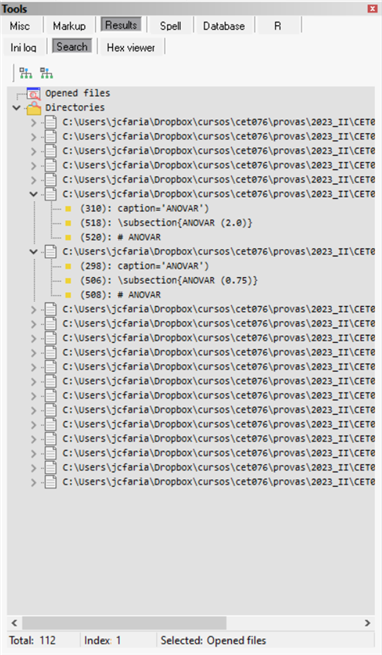
\includegraphics[scale=0.35]{./res/tools_results_search.png}
  \caption{Search (Tools/Results).}
  \label{fig:tools_results_search}
\end{figure}
%-------------------------------------------------------------------------

The interface
(Figure \ref{fig:tools_results_search})
for \textit{Search} results associated with \textit{Search in files}.

The results for the \textit{Search in files} actions are displayed
as a tree with all files. Double click the file to open it in
the editor interface.


%% Hex viewer
%-------------------------------------------------------------------------
\subsubsection{Hex viewer:}\\
\index{tools interface!hex}

\begin{figure}[H]
  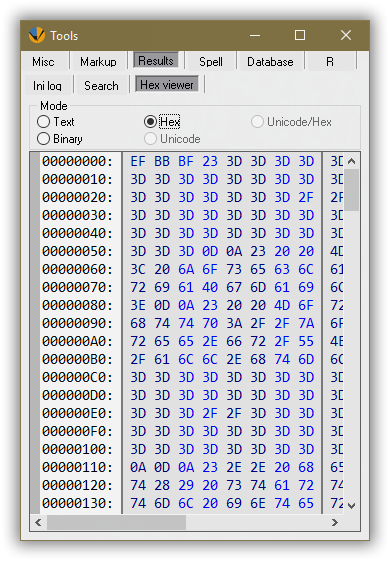
\includegraphics[scale=0.35]{./res/tools_results_hex.png}
  \caption{Hex (Tools/Hex viewer).}
  \label{fig:tools_results_hex}
\end{figure}
%-------------------------------------------------------------------------

The interface
(Figure \ref{fig:tools_results_hex})
for \textit{Hex viewer} results associated to any active file.


%% Spell
%-------------------------------------------------------------------------
\hypertarget{working_tools_spell}{}
\subsection{Spell (Tools)}
\index{tools interface!spell}

\begin{figure}[H]
  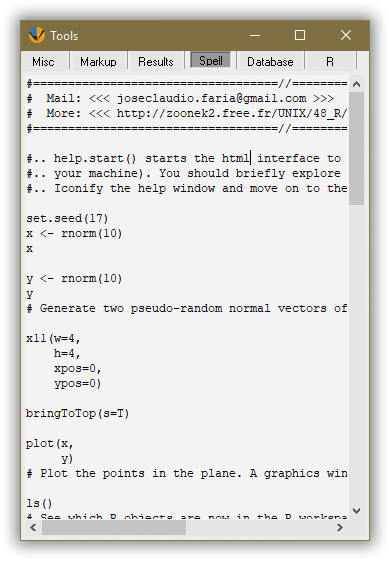
\includegraphics[scale=0.35]{./res/tools_spell.png}
  \caption{Spelling (Tools).}
  \label{fig:tools_spell}
\end{figure}
%-------------------------------------------------------------------------

\begin{footnotesize}
  \begin{tabularx}{\textwidth}{>{\hsize=0.3\hsize}X>{\hsize=0.7\hsize}X}\\
    \hline
    \textbf{Tool} & \textbf{Description} \\
    \hline
    Spell & Interface to speller \\
    \hline
    \\
  \end{tabularx}
\end{footnotesize}

To enable spellchecking with Tinn-R it is necessary to install at
least one dictionary of the list of
\href{http://www.luziusschneider.com/Speller/English/index.htm}{available} ones.
It is also a good idea to install the dictionary manager.
\href{\#configuration\_spellerinstalation}{See instructions ...}.


%% Database
%-------------------------------------------------------------------------
\hypertarget{working_tools_database}{}
\subsection{Database (Tools)}
\index{tools interface!database}

\begin{figure}[H]
  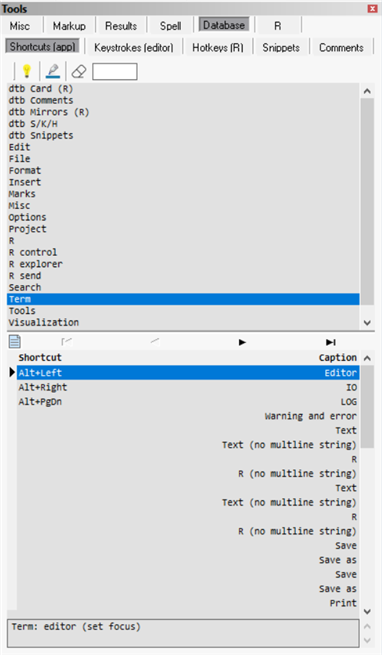
\includegraphics[scale=0.35]{./res/tools_database_shortcuts.png}~~
  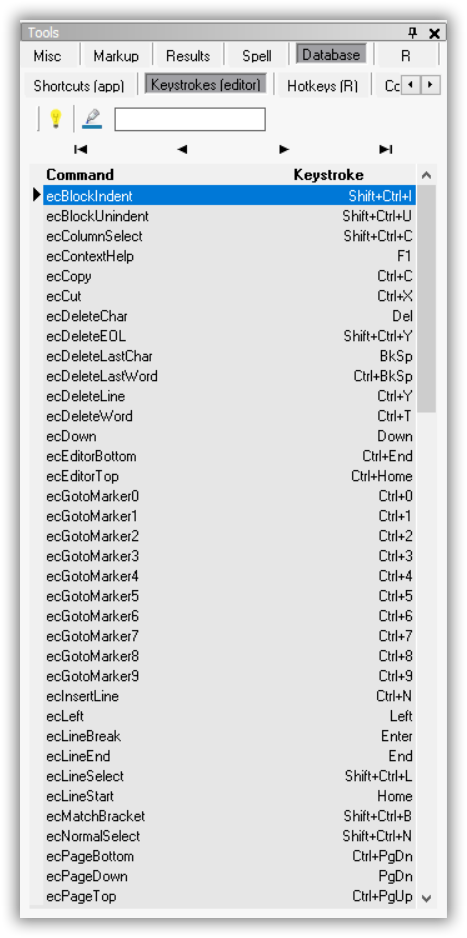
\includegraphics[scale=0.35]{./res/tools_database_keystrokes.png}~~
  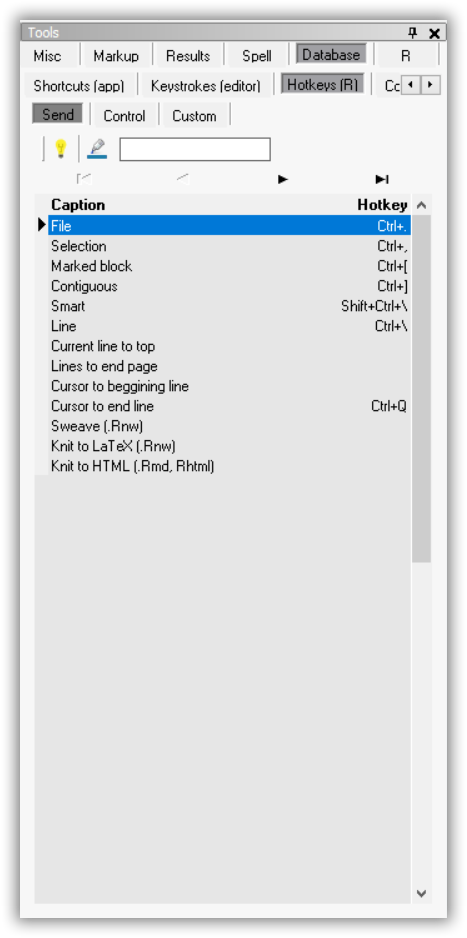
\includegraphics[scale=0.35]{./res/tools_database_rh_send.png}~~
  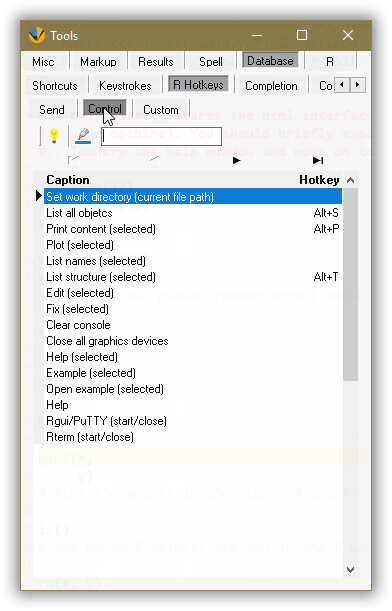
\includegraphics[scale=0.35]{./res/tools_database_rh_control.png}\\
  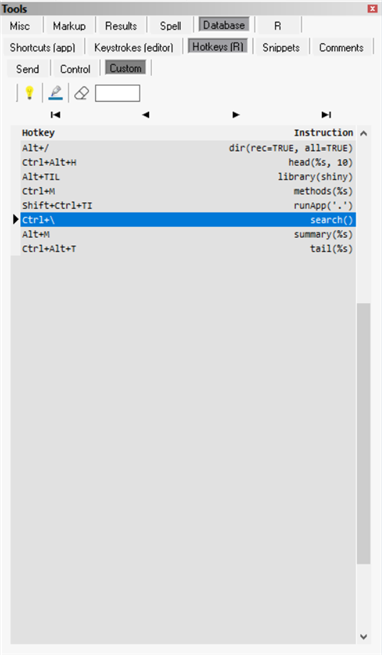
\includegraphics[scale=0.35]{./res/tools_database_rh_custom.png}~~
  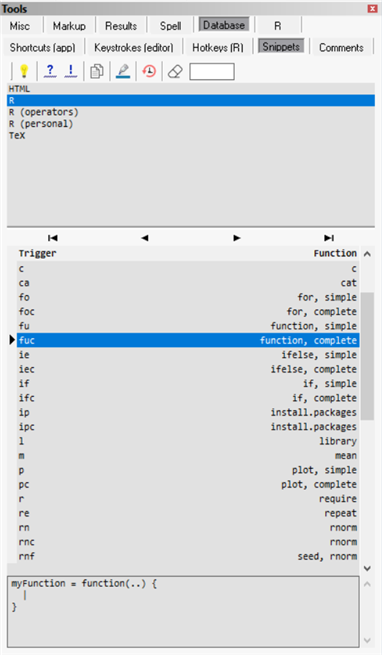
\includegraphics[scale=0.35]{./res/tools_database_snippets.png}~~
  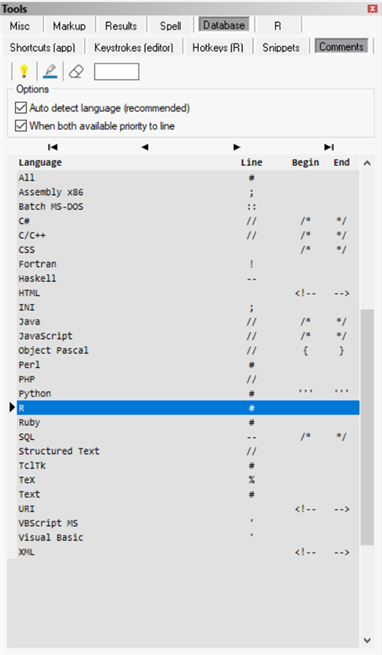
\includegraphics[scale=0.35]{./res/tools_database_comments.png}\\
  \caption{Database (Tools).}
  \label{fig:tools_database}
\end{figure}
%-------------------------------------------------------------------------

\begin{table}
  \begin{footnotesize}
    \begin{tabularx}{\textwidth}{>{\hsize=0.3\hsize}X>{\hsize=0.7\hsize}X}\\
      \hline
      \textbf{Tool} & \textbf{Description} \\
      \hline
      Shortcuts & A digital shortcuts interface based in a XML database \\
      Snippets & A digital snippets interface based in a XML database \\
      Comments & A digital comments interface based in a XML database \\
      \hline
      \\
    \end{tabularx}
  \end{footnotesize}
  \caption{Database (Tools)}
  \label{tab:tools_database}
\end{table}


The database
(Figure \ref{fig:tools_database} and
Table \ref{tab:tools_database})
uses the native XML engine provided by Embarcadero. Each tab
(\textit{Shortcuts}, \textit{Snippets} and
\textit{Comments}) has its own pop-up menus and toolbars.


%% Shortcuts
%-------------------------------------------------------------------------
\subsubsection{Shortcuts:}\\
\index{tools interface!shortcuts}
%-------------------------------------------------------------------------

The \textit{Shortcuts} interface allows the user to find out about
the internal organization of Tinn-R and also to customize all
shortcuts related to the application. It is our intention, in
the near future, to add additional keystrokes related to the
editor and to the \RR{} hotkeys.

The available buttons
(Figure \ref{fig:tools_database})
are:

\begin{quote}
  \begin{footnotesize}
    \begin{description}
      \item[Help:]
        Opens the User guide.
      \item[Edit:]
        Opens the dialog \textit{Snippets dataset (xml based)}.
      \item [Clear:]
        Clears the filter edit box.
    \end{description}
  \end{footnotesize}
\end{quote}

The \textit{Edit} button opens the dialog shown in the Figure \ref{fig:dlg_skh_map_shortcuts}.

%% Keystrokes (editor)
%-------------------------------------------------------------------------
\subsubsection{Keystrokes (editor):}\\
\index{tools interface!Keystrokes (editor)}
%-------------------------------------------------------------------------

This window allows the user to have an overview of the keystrokes related to the SynEdit class
(Editor, IO and LOG). The filter edit box allows you to quickly find shortcuts.

You need to be aware that some shortcuts are superimposed by Shortcuts (app). In these cases,
the shortcuts displayed in this window can be designed and used, for the most part,
as secondary shortcuts for methods of the SynEdit class.

The available buttons
(Figure \ref{fig:tools_database})
are:

\begin{quote}
  \begin{footnotesize}
    \begin{description}
      \item[Help:]
        Opens the User guide.
      \item[Edit:]
        Opens the dialog \textit{Keystrokes (editor) dataset (xml based)}.
      \item [Clear:]
        Clears the filter edit box.
    \end{description}
  \end{footnotesize}
\end{quote}

The \textit{Edit} button opens the dialog shown in the Figure \ref{fig:dlg_skh_map_keystrokes}.


%% Hotkeys
%-------------------------------------------------------------------------
\subsubsection{Hotkeys:}\\
\index{tools interface!Hotkeys}
%-------------------------------------------------------------------------
The main tab called Hotkeys has three daughter tabs: Send, Control and Custom.

The purpose of these windows is to enable quick consultation of each one as well as allowing you
to enter the editing modes for each one. The filter edit box makes it easy to find hotkeys.

Hotkeys are very interesting resources to use when communicating with \RR{}, since the triggered action
is independent of whether or not the focus is in the Tinn-R interface and whether it is is
also independent of the location.

Read more about the subject at:
\begin{itemize}
  \item \href{\#faq\_hotkeys}{FAQ: Hotkeys}
  \item \href{\#dlg\_hotkeys\_editor}{Hotkeys: editor}
  \item \href{\#secrets\_after\_installation}{Some Secrets for an Efficient Use}
\end{itemize}

The available buttons
(Figure \ref{fig:tools_database})
are:

\begin{quote}
  \begin{footnotesize}
    \begin{description}
      \item[Help:]
        Opens the User guide.
      \item[Edit:]
        Opens the dialog \textit{Hotkeys dataset (xml based)}.
      \item [Clear:]
        Clears the filter edit box.
    \end{description}
  \end{footnotesize}
\end{quote}

The \textit{Edit} button opens the dialog shown in the Figure \ref{fig:dlg_skh_map_hotkeys}.


%% Snippets
%-------------------------------------------------------------------------
\subsubsection{Snippets:}\\
\index{tools interface!snippets}
%-------------------------------------------------------------------------

The \textit{Snippet} resource is very simple and allows high level
of user customization related to edition.

This resource adds a granular level of user customization for editing
all within Tinn-R.

The snippets (database based) allows the user to add functions based
on several programming languages such as \RR{}, \TeX, among others.

The available buttons
(Figure \ref{fig:tools_database})
are:

\begin{quote}
  \begin{footnotesize}
    \begin{description}
      \item[Help:]
        Sends the following instruction to \RR{}: \texttt{help('selected function')}.
      \item[Example:]
        Sends the following instruction to \RR{}:
        \texttt{example('selected function')}.
      \item[Copy function:]
        Places the selected function in the clipboard.
      \item[Copy description:]
        Places the description of the selected function in the clipboard.
      \item[Edit:]
        Opens the dialog \textit{Snippets dataset (xml based)} below.
      \item[Insert:]
        Inserts the selected function in the active editor. A \texttt{Double click}
        or \texttt{Enter} performs the same function.
        The default shortcut is \texttt{CTRL + J}, but this can be customized under
        \textit{Options/Shortcuts} or \textit{Tools/Database/Shortcuts}. To use
        it just push the keystrokes after any valid word:

        \begin{verbatim}
          if<CTRL + J> to obtain:
          if (| < )

          ifc<CTRL + J> to obtain:
          if (| < ) {

          }

          fo<CTRL + J> to obtain:
          for (i in 1:i|)

          foc<CTRL + J> to obtain:
          for (i in 1:|) {

          }

          sw<CTRL + J> to obtain:
          switch(|,
          a = ' ',
          b = ' ',
          )

          wh<CTRL + J> to obtain:
          i = 0
          while (i < |) {

            i = i + 1
          }

          eq<CTRL + J> to obtain:
          \begin{equation}\label{eq_01}
            |
          \end{equation}
        \end{verbatim}

        \subsubsection{Observations:}\\
        \index{Snippets}
        \begin{enumerate}
          \item Only two letters were used to define the functions (for example:
            \textit{fo} = \textit{for}, \textit{fu} = \textit{function});
          \item Therefore, we added the letter \texttt{c} for more complex
            structures (for example: \textit{foc}, \textit{fuc});
          \item The \texttt{$|$} symbol is used to define where the cursor
            will first stop after snippets. After being selected
            the \texttt{$|$} symbol marks the point where the user can start
            typing.
        \end{enumerate}
      \item [Clear:]
        Clears the filter edit box.
    \end{description}
  \end{footnotesize}
\end{quote}

The \textit{Edit} button opens the dialog showed in the Figure \ref{fig:dlg_snippets}.


%% Comments
%-------------------------------------------------------------------------
\subsubsection{Comments:}\\
\index{tools interface!Comments}
%-------------------------------------------------------------------------

The \textit{Comments} resource is very simple and allows high level
of user customization.

From version 3.0.1.0 Tinn-R automatically recognizes the
language of the file on focus. Further, inside the file
- if it is a syntax a multi-highlighter (complex syntax) - which language of
the line where the cursor (or selection) is found.

This identification is done automatically if (and only if) the option
\textit{(x) Auto detect language (recomended)} is checked. Otherwise
the user is forcing the application to use the comments of the selected language
(indicator arrow).

Selected code snippets involving more than one language will not be commented/uncommented
and a warning message is issued. That is, you must select only the snippet of a single language.

The available buttons
(Figure \ref{fig:tools_database})
are:

\begin{quote}
  \begin{footnotesize}
    \begin{description}
      \item[Help:]
        It opens the \textit{User Guide} on the section Database.
      \item[Edit:]
        It opens the dialog \textit{R card dataset (xml based)}.
      \item [Clear:]
        Clears the filter edit box.
    \end{description}
  \end{footnotesize}
\end{quote}

The \textit{Edit} button opens the dialog shown in the Figure \ref{fig:dlg_comments}.


%% R
%-------------------------------------------------------------------------
\hypertarget{working_tools_r}{}
\subsection{R (Tools)}
\index{tools interface!R}

\begin{figure}[H]
  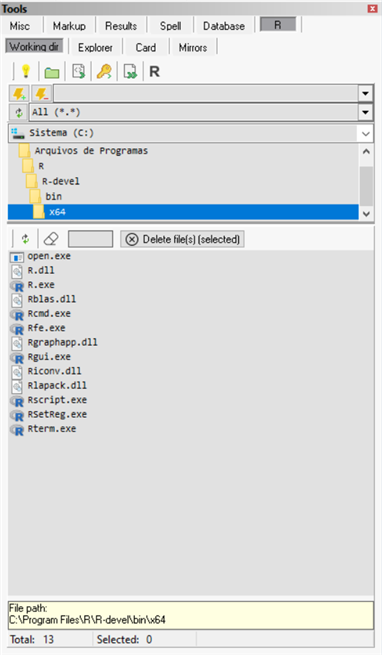
\includegraphics[scale=0.35]{./res/tools_r_workingdir.png}~~
  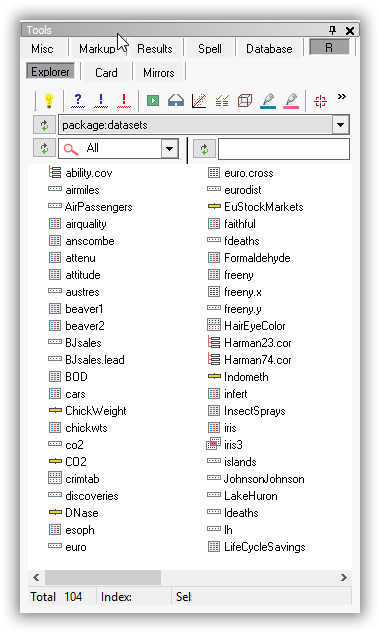
\includegraphics[scale=0.35]{./res/tools_r_explorer.png}~~
  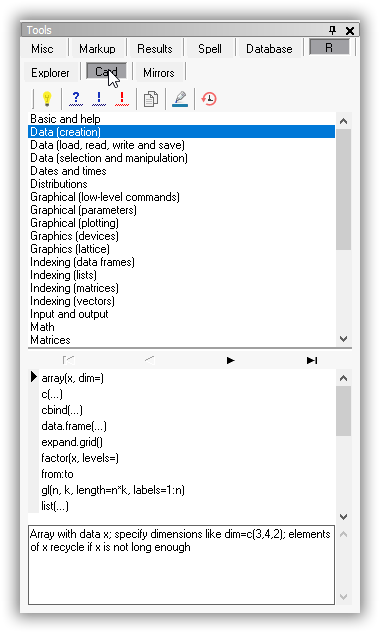
\includegraphics[scale=0.35]{./res/tools_r_card.png}~~
  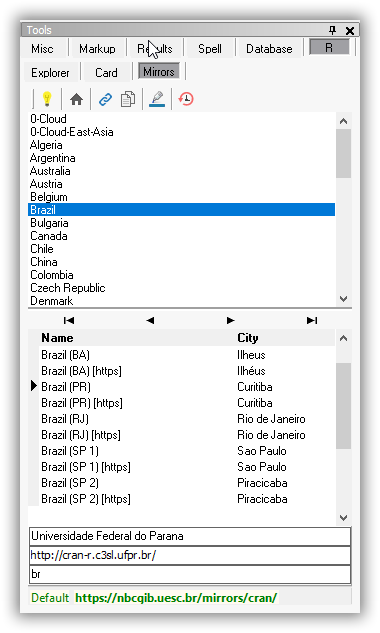
\includegraphics[scale=0.35]{./res/tools_r_mirrors.png}\\
  \caption{R (Tools).}
  \label{fig:tools_r}
\end{figure}
%-------------------------------------------------------------------------

\begin{table}
  \begin{footnotesize}
    \begin{tabularx}{\textwidth}{>{\hsize=0.3\hsize}X>{\hsize=0.7\hsize}X}\\
      \hline
      \textbf{Tool} & \textbf{Description} \\
      \hline
      Working dir & A graphical interface to make it easy to deal with the \RR{} interpreter's Working Directory \\
      Explorer & Simple and functional graphical interface of objects of the \RR{} environment \\
      Card & A digital and simple \RR{} card based in a XML database \\
      Mirrors & A digital and simple \RR{} mirrors management based in a XML database \\
      \hline
      \\
    \end{tabularx}
  \end{footnotesize}
  \caption{R (Tools).}
  \label{tab:tools_r}
\end{table}

A simple and functional graphical interface
(Figure \ref{fig:tools_r} and
Table \ref{tab:tools_r})
of objects, card and mirrors management of the \RR{} environment.


%% Working dir
%-------------------------------------------------------------------------
\subsubsection{Working dir:}\\
\index{tools interface!Working dir}
\index{R!Working dir}
%-------------------------------------------------------------------------

This interface
(Figure \ref{fig:tools_r})
allows a graphical visualization of the active \RR{} working directory. It also
allows storing favorites and indicating the work folder to \RR{} with
several interesting options.

This interface is experimental, but we believe it is of great importance for novice users.


%% Explorer
%-------------------------------------------------------------------------
\subsubsection{Explorer:}\\
\index{tools interface!R explorer}
\index{R!explorer}
\index{R explorer}
%-------------------------------------------------------------------------

This interface
(Figure \ref{fig:tools_r})
has its own pop-up menu, toolbar and three combo box. The
pop-up menu and toolbar contain the most common actions related to an object
explorer.

The button \textit{R explorer: refresh environment} sends an instruction to
\RR{} environment requesting the list of all loaded packages in the current
session. The result is shown inside a graphical classified list. When one
of these is selected, the graphical list (and structure) of the objects
are shown.

There are two options of filter: type of objects and any sequence of
characters associated with the names of the objects.

It is possible to remove visible objects of the user workspace (.GlobalEnv)
using the key \textit{Delete}. To do this, select an object and type
\textit{Delete}.

A double click in any selected object will add its name to the editor.
If the object is dragged to the editor interface, the textual description
of the object is always shown in a new file. It is useful to know the
sources of functions and to see data objects (vectors, frames, list, etc).

If view mode is grid, you can see more details about each object. In grid mode,
in the \textit{Dim} column, the description \textbf{ns} and \textbf{nd} mean
nonsense and undefined, respectively.

%% Card
%-------------------------------------------------------------------------
\subsubsection{Card:}\\
\index{tools interface!card (R)}
\index{R!card}
%-------------------------------------------------------------------------

The \textit{card} was based on two \RR{} cards already published:
R/Rpad Reference Card by Tom Short and \RR{} reference card by Jonathan Baron.

\begin{figure}[H]
  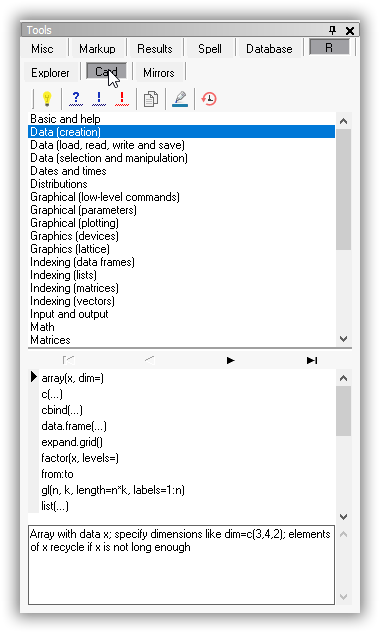
\includegraphics[scale=0.35]{./res/tools_r_card.png}\\
  \caption{R card (dataset).}
  \label{fig:tools_r_card}
\end{figure}

The available buttons
(Figure \ref{fig:tools_r_card})
are:

\begin{quote}
  \begin{footnotesize}
    \begin{description}
      \item[Help:]
        Sends the following instruction to \RR{}: \texttt{help('selected function')}.
      \item[Example:]
        Sends the following instruction to \RR{}: \texttt{example('selected function')}.
      \item[Copy function:]
        Places the selected function in the clipboard.
      \item[Copy descrition:]
        Places the descrition of the selected function on the clipboard.
      \item[Edit:]
        Opens the dialog \textit{R card dataset (xml based)} below.
      \item[Insert:]
        Inserts the selected function in the active editor. A
        \texttt{Double click} or \texttt{Enter} performs the same function.
      \item [Clear:]
        Clears the filter edit box.
    \end{description}
  \end{footnotesize}
\end{quote}

The \textit{Edit} button opens the dialog shown in the Figure \ref{fig:dlg_r_card}.


%% Mirrors
%-------------------------------------------------------------------------
\subsubsection{Mirrors:}\\
\index{tools interface!mirrors (R)}
\index{R!mirrors}
%-------------------------------------------------------------------------

The \textit{Mirrors} is an interface that allows the user to manage the repositories (or mirrors) of \RR{}.
You should always choose a repository physically closest to where you are,
so that, the Web communication tends to be faster and more efficient.

The default mirror is the University \href{http://cran.at.r-project.org/}{Wien}
(Austria). Consider that this is the central mirror of CRAN.

The reasons for the Tinn-R always set a repository are two:
\begin {itemize}
   \item Prevent \RR{} keep asking which repository you want to use in each session;
   \item Workaround of intermittency (only Rterm.exe) display the dialog for selecting the repository.
    That is, sometimes the dialog is displayed and not others. The cause of this intermittency is still unknown.
\end {itemize}

\begin{figure}[H]
  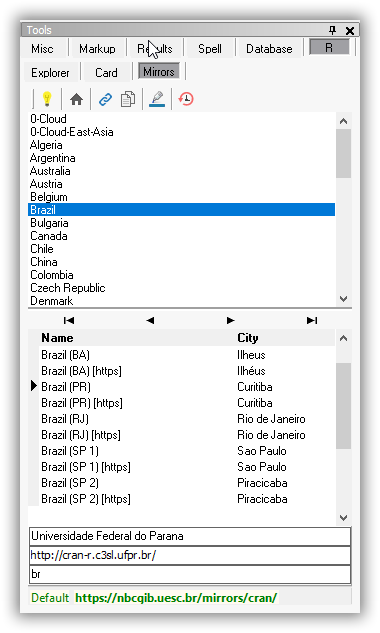
\includegraphics[scale=0.35]{./res/tools_r_mirrors.png}\\
  \caption{R mirrors (dataset).}
  \label{fig:tools_dlg_mirrors}
\end{figure}

The available buttons
(Figure \ref{fig:tools_dlg_mirrors})
are:

\begin{quote}
  \begin{footnotesize}
    \begin{description}
      \item[Help:]
        Opens the User guide.
      \item[Update:]
        Updates the available \RR{} mirrors.
      \item[Copy host:]
        Places the selected mirror host in the clipboard.
      \item[Copy URL:]
        Places the selected mirror URL in the clipboard.
      \item[Edit:]
        Opens the dialog \textit{R mirrors (xml based)} below.
      \item[Insert:]
        Sends the following instruction to \RR{}: \texttt{options('repos='URL of selected mirror')}.
      \item [Clear:]
        Clears the filter edit box.
    \end{description}
  \end{footnotesize}
\end{quote}

The \textit{Edit} button opens the dialog shown in the Figure \ref{fig:dlg_mirrors}.
